\begin{tikzpicture}
    \node at (0,6){
        \begin{tikzpicture}
            \foreach \iangle in {45,80,120,150}{
                    \fill[fill=orange!60!red,fill opacity=0.2](0,0) -- (0:2) arc (0:\iangle:2) -- cycle;
                    \filldraw[fill=green!40!black,fill opacity=0.5](0,0) --(0:0.3) arc (0:\iangle:0.3) -- cycle;
                    \draw[->] (-2.2,0) -- (2.2,0);
                    \draw[->] (0,-2.2) -- (0,2.2);
                    \draw[thick,draw=green!40!black] (0,0) circle (2);
                    \coordinate[label=\iangle:$P$] (P) at (\iangle:2);
                    \coordinate[label=below:$P_0$] (P0) at (P |- 0,0);
                    \draw (0,0) -- (P);
                    \draw (P) -- (P0);
                    \draw[->] (5,0) -- (11,0);
                    \draw[->] (0,-2.2) -- (0,2.2);
                    \draw[->] (2*pi,-2.2) -- (2*pi,2.2);
                    \draw[thick,domain=4:10,smooth,draw=green!40!black] plot(\x,{2*sin(\x r)}) node[right] {$\sin x$};
                    \foreach \y in {-1,1} {\draw (-0.05,\y) -- (0.05,\y); }
                    \coordinate[label=above:$Q$] (Q) at ({rad(\iangle+360)},{2*sin(\iangle+360)});
                    \coordinate[label=below:$Q_0$] (Q0) at (Q |- 0,0);
                    \draw (Q) -- (Q0);
                    \draw[dashed] (P) -- (Q);
                }
        \end{tikzpicture}};

    \node at (0,0){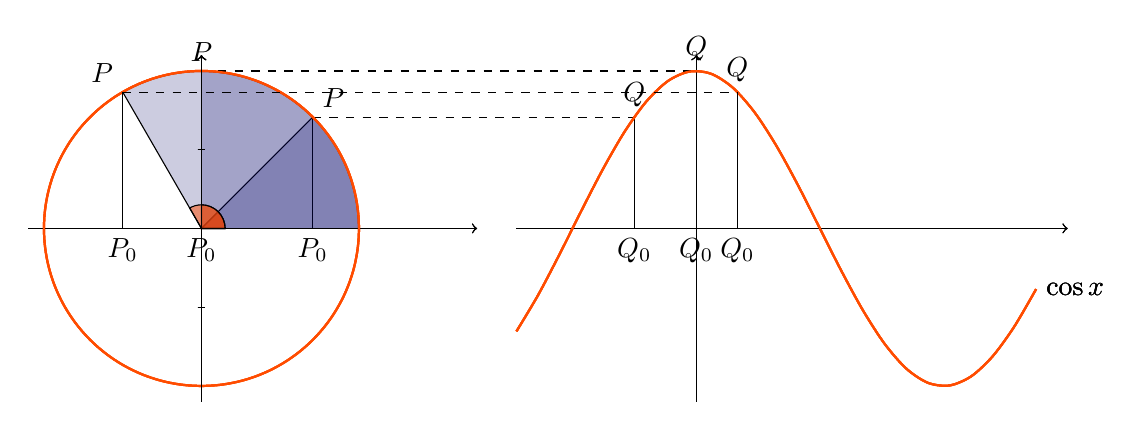
\begin{tikzpicture}
            \foreach \iangle in {45,90,120}{
                    \fill[fill=blue!40!black,fill opacity=0.2](0,0) -- (0:2) arc (0:\iangle:2) -- cycle;
                    \filldraw[fill=orange!60!red,fill opacity=0.5](0,0) --(0:0.3) arc (0:\iangle:0.3) -- cycle;
                    \draw[->] (-2.2,0) -- (3.5,0);
                    \draw[->] (0,-2.2) -- (0,2.2);
                    \draw[thick,draw=orange!60!red] (0,0) circle (2);
                    \coordinate[label=\iangle:$P$] (P) at (\iangle:2);
                    \coordinate[label=below:$P_0$] (P0) at (P |- 0,0);
                    \draw (0,0) -- (P);
                    \draw (P) -- (P0);
                    \draw[->] (4,0) -- (11,0);
                    \draw[->] (0,-2.2) -- (0,2.2);
                    \draw[->] (2*pi,-2.2) -- (2*pi,2.2);
                    \draw[thick,domain=4:10.6,smooth,draw=orange!60!red] plot(\x,{2*cos(\x r)}) node[right] {$\cos x$};
                    \foreach \y in {-1,1} {\draw (-0.05,\y) -- (0.05,\y);}
                    \coordinate[label=above:$Q$] (Q) at ({rad(\iangle+270)},{2*cos(\iangle+270)});
                    \coordinate[label=below:$Q_0$] (Q0) at (Q |- 0,0);
                    \draw (Q) -- (Q0);
                    \draw[dashed] (P) -- (Q);
                }
        \end{tikzpicture}};
\end{tikzpicture}

\subsection{正余弦函数的图像}

\begin{tikzpicture}
    \begin{axis}[
            title={三角函数图像},
            axis lines=middle,
            xlabel={$x$},
            ylabel={$y$},
            grid=major,
            enlargelimits=false,
            % 使用表达式定义x轴刻度，更精确且易读
            xtick={-pi, -pi/2, 0, pi/2, pi, 3*pi/2, 2*pi, 5*pi/2, 3*pi},
            xticklabels={
                    $-\pi$,
                    $-\frac{\pi}{2}$,
                    $0$,
                    $\frac{\pi}{2}$,
                    $\pi$,
                    $\frac{3\pi}{2}$,
                    $2\pi$,
                    $\frac{5\pi}{2}$,
                    $3\pi$
                },
            ytick={-3,-2,-1,0,1,2,3},
            ymin=-3.5, ymax=3.5, % 设置y轴范围
            samples=101,
            legend pos=outer north east, % 将图例放在右上角外部
            legend cell align={left}
        ]

        % sin(x)
        \addplot[blue, no marks, domain=-pi:3*pi, thick] {sin(deg(x))};
        \addlegendentry{$\sin(x)$}

        % cos(x)
        \addplot[red, no marks, domain=-pi:3*pi, thick] {cos(deg(x))};
        \addlegendentry{$\cos(x)$}

        % tan(x)
        % pgfplots 会自动处理不连续点，设置 `unbounded coords=jump` 即可
        \addplot[orange, no marks, domain=-pi:3*pi, thick, unbounded coords=jump] {tan(deg(x))};
        \addlegendentry{$\tan(x)$}

        % 为 tan(x) 绘制渐近线
        \draw[orange, dashed] (axis cs:-pi/2, \pgfkeysvalueof{/pgfplots/ymin}) -- (axis cs:-pi/2, \pgfkeysvalueof{/pgfplots/ymax});
        \draw[orange, dashed] (axis cs:pi/2,  \pgfkeysvalueof{/pgfplots/ymin}) -- (axis cs:pi/2,  \pgfkeysvalueof{/pgfplots/ymax});
        \draw[orange, dashed] (axis cs:3*pi/2,\pgfkeysvalueof{/pgfplots/ymin}) -- (axis cs:3*pi/2,\pgfkeysvalueof{/pgfplots/ymax});
        \draw[orange, dashed] (axis cs:5*pi/2,\pgfkeysvalueof{/pgfplots/ymin}) -- (axis cs:5*pi/2,\pgfkeysvalueof{/pgfplots/ymax});

    \end{axis}
\end{tikzpicture}

% ==========================================================
\section{$y=\sin x$ 的图像与性质}
% ==========================================================

\begin{figure}[ht]
    \centering
    \begin{tikzpicture}[scale=0.8]
        \draw[->, >=Stealth] (-2.5*pi, 0) -- (2.5*pi, 0) node[below] {$x$};
        \draw[->, >=Stealth] (0, -1.5) -- (0, 1.5) node[left] {$y$};
        \node[below left] at (0,0) {$O$};

        % 关键点
        \foreach \x/\xtext in {-2*pi/$-2\pi$, -3*pi/2/$-\frac{3\pi}{2}$, -pi/$-\pi$, -pi/2/$-\frac{\pi}{2}$, pi/2/$\frac{\pi}{2}$, pi/$\pi$, 3*pi/2/$\frac{3\pi}{2}$, 2*pi/$2\pi$} {
                \fill (\x,0) circle[radius=1.5pt] node[below] {\xtext};
            }

        % 函数图像
        \draw[smooth, thick, samples=100, blue, domain=-2.5*pi:2.5*pi] plot(\x, {sin(\x r)});
    \end{tikzpicture}
    \caption{$y=\sin x$ 的函数图像}
\end{figure}

\begin{table}[ht]
    \centering
    \caption{$y=\sin x$ 的性质}
    \renewcommand{\arraystretch}{1.5} % 增加行高
    \begin{tabular}{c|c|l}
        \toprule[1.5pt]
        \multicolumn{2}{c|}{\textbf{性质}} & \multicolumn{1}{c}{\textbf{描述}}                                                                             \\
        \midrule
        \multicolumn{2}{c|}{定义域}         & $\mathbb{R}$                                                                                                \\
        \midrule
        \multicolumn{2}{c|}{值域}          & $[-1,1]$                                                                                                    \\
        \midrule
        \multirow{2}{*}{最值}              & 最大值                             & 当 $x=\frac{\pi}{2}+2k\pi \ (k\in \mathbb{Z})$ 时, $y_{\max}=1$             \\
        \cmidrule{2-3}
                                         & 最小值                             & 当 $x=\frac{3\pi}{2}+2k\pi \ (k\in \mathbb{Z})$ 时, $y_{\min}=-1$           \\
        \midrule
        \multicolumn{2}{c|}{周期性 (最小正周期)} & $T=2\pi$                                                                                                    \\
        \midrule
        \multirow{2}{*}{单调性}             & 单调递增区间                          & $\left[-\frac{\pi}{2}+2k\pi, \frac{\pi}{2}+2k\pi\right], k\in \mathbb{Z}$ \\
        \cmidrule{2-3}
                                         & 单调递减区间                          & $\left[\frac{\pi}{2}+2k\pi, \frac{3\pi}{2}+2k\pi\right], k\in \mathbb{Z}$ \\
        \midrule
        \multirow{2}{*}{对称性}             & 对称中心                            & $\left(k\pi, 0\right), k\in \mathbb{Z}$                                   \\
        \cmidrule{2-3}
                                         & 对称轴                             & 直线 $x=\frac{\pi}{2}+k\pi, k\in \mathbb{Z}$                                \\
        \bottomrule[1.5pt]
    \end{tabular}
\end{table}

\clearpage

% ==========================================================
\section{$y=\cos x$ 的图像与性质}
% ==========================================================

\begin{figure}[ht]
    \centering
    \begin{tikzpicture}[scale=0.8]
        \draw[->, >=Stealth] (-2.5*pi, 0) -- (2.5*pi, 0) node[below] {$x$};
        \draw[->, >=Stealth] (0, -1.5) -- (0, 1.5) node[left] {$y$};
        \node[below left] at (0,0) {$O$};

        % 关键点
        \foreach \x/\xtext in {-2*pi/$-2\pi$, -3*pi/2/$-\frac{3\pi}{2}$, -pi/$-\pi$, -pi/2/$-\frac{\pi}{2}$, pi/2/$\frac{\pi}{2}$, pi/$\pi$, 3*pi/2/$\frac{3\pi}{2}$, 2*pi/$2\pi$} {
                \fill (\x,0) circle[radius=1.5pt] node[below] {\xtext};
            }

        % 函数图像
        \draw[smooth, thick, samples=100, red, domain=-2.5*pi:2.5*pi] plot(\x, {cos(\x r)});
    \end{tikzpicture}
    \caption{$y=\cos x$ 的函数图像}
\end{figure}

\begin{table}[ht]
    \centering
    \caption{$y=\cos x$ 的性质}
    \renewcommand{\arraystretch}{1.5}
    \begin{tabular}{c|c|l}
        \toprule[1.5pt]
        \multicolumn{2}{c|}{\textbf{性质}} & \multicolumn{1}{c}{\textbf{描述}}                                                         \\
        \midrule
        \multicolumn{2}{c|}{定义域}         & $\mathbb{R}$                                                                            \\
        \midrule
        \multicolumn{2}{c|}{值域}          & $[-1,1]$                                                                                \\
        \midrule
        \multirow{2}{*}{最值}              & 最大值                             & 当 $x=2k\pi \ (k\in \mathbb{Z})$ 时, $y_{\max}=1$       \\
        \cmidrule{2-3}
                                         & 最小值                             & 当 $x=\pi+2k\pi \ (k\in \mathbb{Z})$ 时, $y_{\min}=-1$  \\
        \midrule
        \multicolumn{2}{c|}{周期性 (最小正周期)} & $T=2\pi$                                                                                \\
        \midrule
        \multirow{2}{*}{单调性}             & 单调递增区间                          & $\left[\pi+2k\pi, 2\pi+2k\pi\right], k\in \mathbb{Z}$ \\
        \cmidrule{2-3}
                                         & 单调递减区间                          & $\left[2k\pi, \pi+2k\pi\right], k\in \mathbb{Z}$      \\
        \midrule
        \multirow{2}{*}{对称性}             & 对称中心                            & $\left(\frac{\pi}{2}+k\pi, 0\right), k\in \mathbb{Z}$ \\
        \cmidrule{2-3}
                                         & 对称轴                             & 直线 $x=k\pi, k\in \mathbb{Z}$                          \\
        \bottomrule[1.5pt]
    \end{tabular}
\end{table}

\clearpage

% ==========================================================
\section{$y=A\sin(\omega x+\phi)$ 的性质}
% ==========================================================

\subsubsection*{$y=A\sin(\omega x+\phi)\ (A>0, \omega>0)$ 的基本概念}
\begin{table}[ht]
    \centering
    \caption{五大基本概念}
    \renewcommand{\arraystretch}{1.5}
    \begin{tabular}{c|c|c|c|c}
        \toprule[1.5pt]
        \textbf{振幅} & \textbf{周期}             & \textbf{频率}                         & \textbf{相位}     & \textbf{初相} \\
        \midrule
        $A$         & $T=\frac{2\pi}{\omega}$ & $f=\frac{1}{T}=\frac{\omega}{2\pi}$ & $\omega x+\phi$ & $\phi$      \\
        \bottomrule[1.5pt]
    \end{tabular}
\end{table}

\subsubsection*{性质求解方法 (换元法)}
求解 $y=A\sin(\omega x+\phi)$ 的相关性质时，核心思想是整体换元。令 $X=\omega x+\phi$，然后将其性质与 $y=A\sin X$ 对比求解。

\begin{table}[ht]
    \centering
    \caption{性质求解核心}
    \renewcommand{\arraystretch}{1.5}
    \begin{tabular}{l|l}
        \toprule[1.5pt]
        \textbf{性质} & \textbf{求解方法}                                                        \\
        \midrule
        单调性         & 将 $\omega x+\phi$ 整体代入 $y=\sin X$ 的单调区间内求解不等式。                       \\
        \midrule
        对称轴         & 令 $\omega x+\phi = \frac{\pi}{2}+k\pi \ (k\in \mathbb{Z})$，反解出 $x$。  \\
        \midrule
        对称中心        & 令 $\omega x+\phi = k\pi \ (k\in \mathbb{Z})$，反解出 $x$，对称中心为 $(x, 0)$。 \\
        \bottomrule[1.5pt]
    \end{tabular}
\end{table}
